% Bei Bedarf können andere Diagramm (ER-Diagramme, Paketdiagramme, endliche Automaten,...) eingesetzt werden, um bestimmte Teile des Programms zu beschreiben.
\section{ER-Modell der DB}
\begin{figure}[h!]
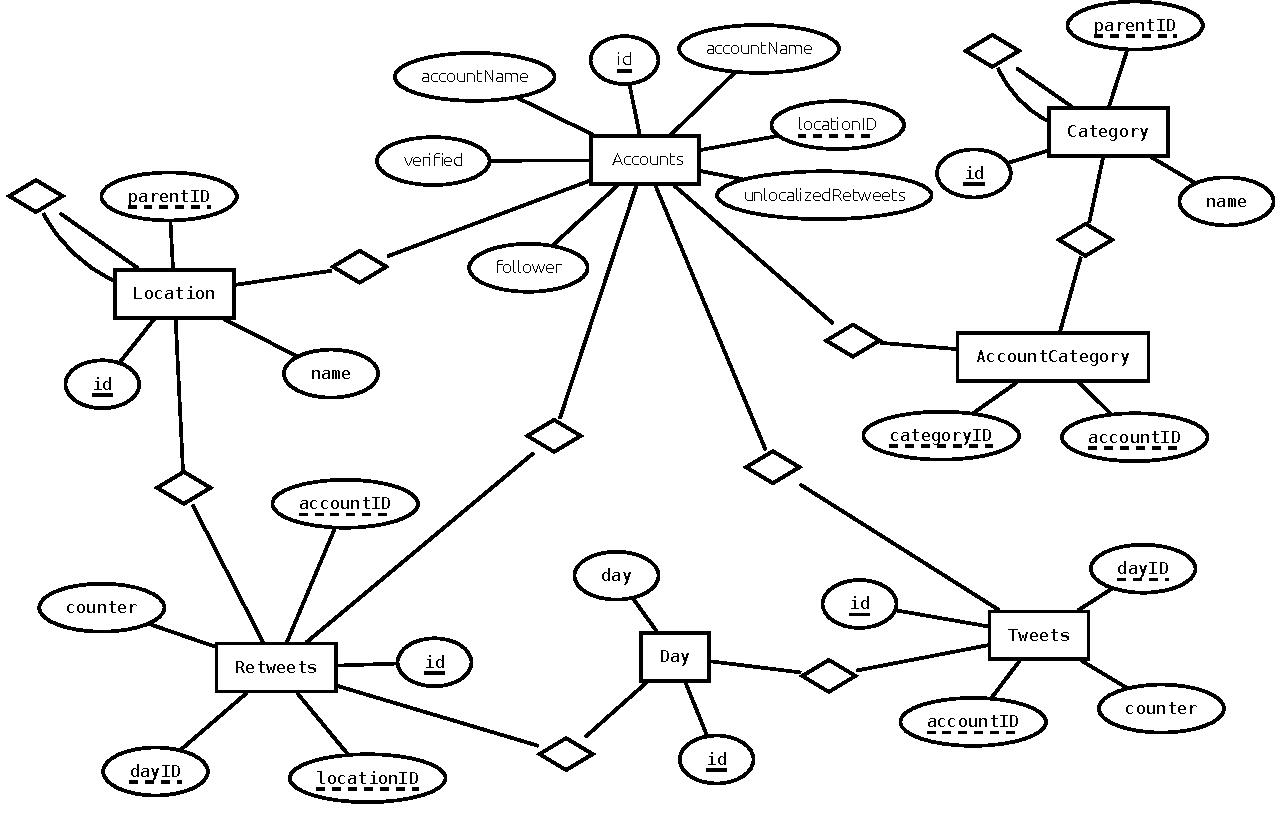
\includegraphics[width=\textwidth,height=\textheight, keepaspectratio=true]{dia/er}
\caption{ER-Modell der MySQL-Datenbank}
\label{fig:mysql-er}
\end{figure}
